

We investigate whether the tokens learned by the first RVQ quantizer
relate to phonetic information.
Utilizing \method or EnCodec, we derive speech tokens from the TIMIT training set and extract the RVQ-1 tokens, denoted as $q_1$. We then compute the conditional probability $p(phoneme|q_1)$ based on the co-occurrence
between phonemes and the codes. The alignments are constructed by selecting the phoneme that occurs most frequently in the receptive field for each $q_1$.

% Figure~\ref{fig:phone_purity} illustrates the $p(phoneme|q_1)$ for both \method and EnCodec. For \method, it's evident that in the codebook of RVQ-1 quantizer, many discrete codes seem to specialize in capturing specific phonetic sounds,  indicating RVQ-1 quantizer can obtain a good alignment between
% codes and labeled phonemes. However, for EnCodec, this phenomenon is not as obvious, and there are cases where many codes in the codebook are underutilized. 
Figure~\ref{fig:phone_purity} visualizes the conditional probability $p(\text{phoneme}|q_1)$ for both \method and EnCodec. A darker color block indicates a higher $p(\text{phoneme}|q_1)$. 
% Consequently, a greater contrast between the diagonal color band and the surrounding area denotes higher phoneme purity, implying a more pronounced mapping from code to phoneme correspondence. 
A more distinct contrast between the diagonal color band and its surrounding area signifies greater phoneme purity, which in turn suggests a more accurate mapping between the code and its corresponding phoneme.
For \method, it's evident that in the codebook of RVQ-1 quantizer, many discrete codes seem to specialize in capturing specific phonetic sounds, indicating RVQ-1 quantizer can obtain a good alignment between codes and labeled phonemes. However, for EnCodec, this phenomenon is not as obvious.

Additionally, Figure~\ref{fig:phone_purity} also reveals that over 600 codes from the EnCodec RVQ-1 codebook have never been utilized, suggesting a suboptimal utilization rate of the codebook when EnCodec encodes speech. A lower utilization rate of the codebook implies that more RVQ layers are required to ensure the quality of synthesized speech, consequently necessitating the generation of more codes during the construction of a spoken generative language model, resulting in greater space, time and computation power consumption.

We further evaluate the models using Phone-Normalized Mutual Information (PNMI) ~\citep{hsu2021hubert}. As shown in Table~\ref{tab:pnmi}, RVQ-1 tokens of \method achieve a superior PNMI score to that of HuBERT units and significantly outperforms EnCodec-RVQ-1. This suggests that the semantic distillation process in \method is effective, thereby explaining its enhanced text alignment performance.



\begin{figure*}[h] 
    % \setlength{\abovecaptionskip}{-0.cm}
    % \setlength{\belowcaptionskip}{-0.5cm}
    \centering 
    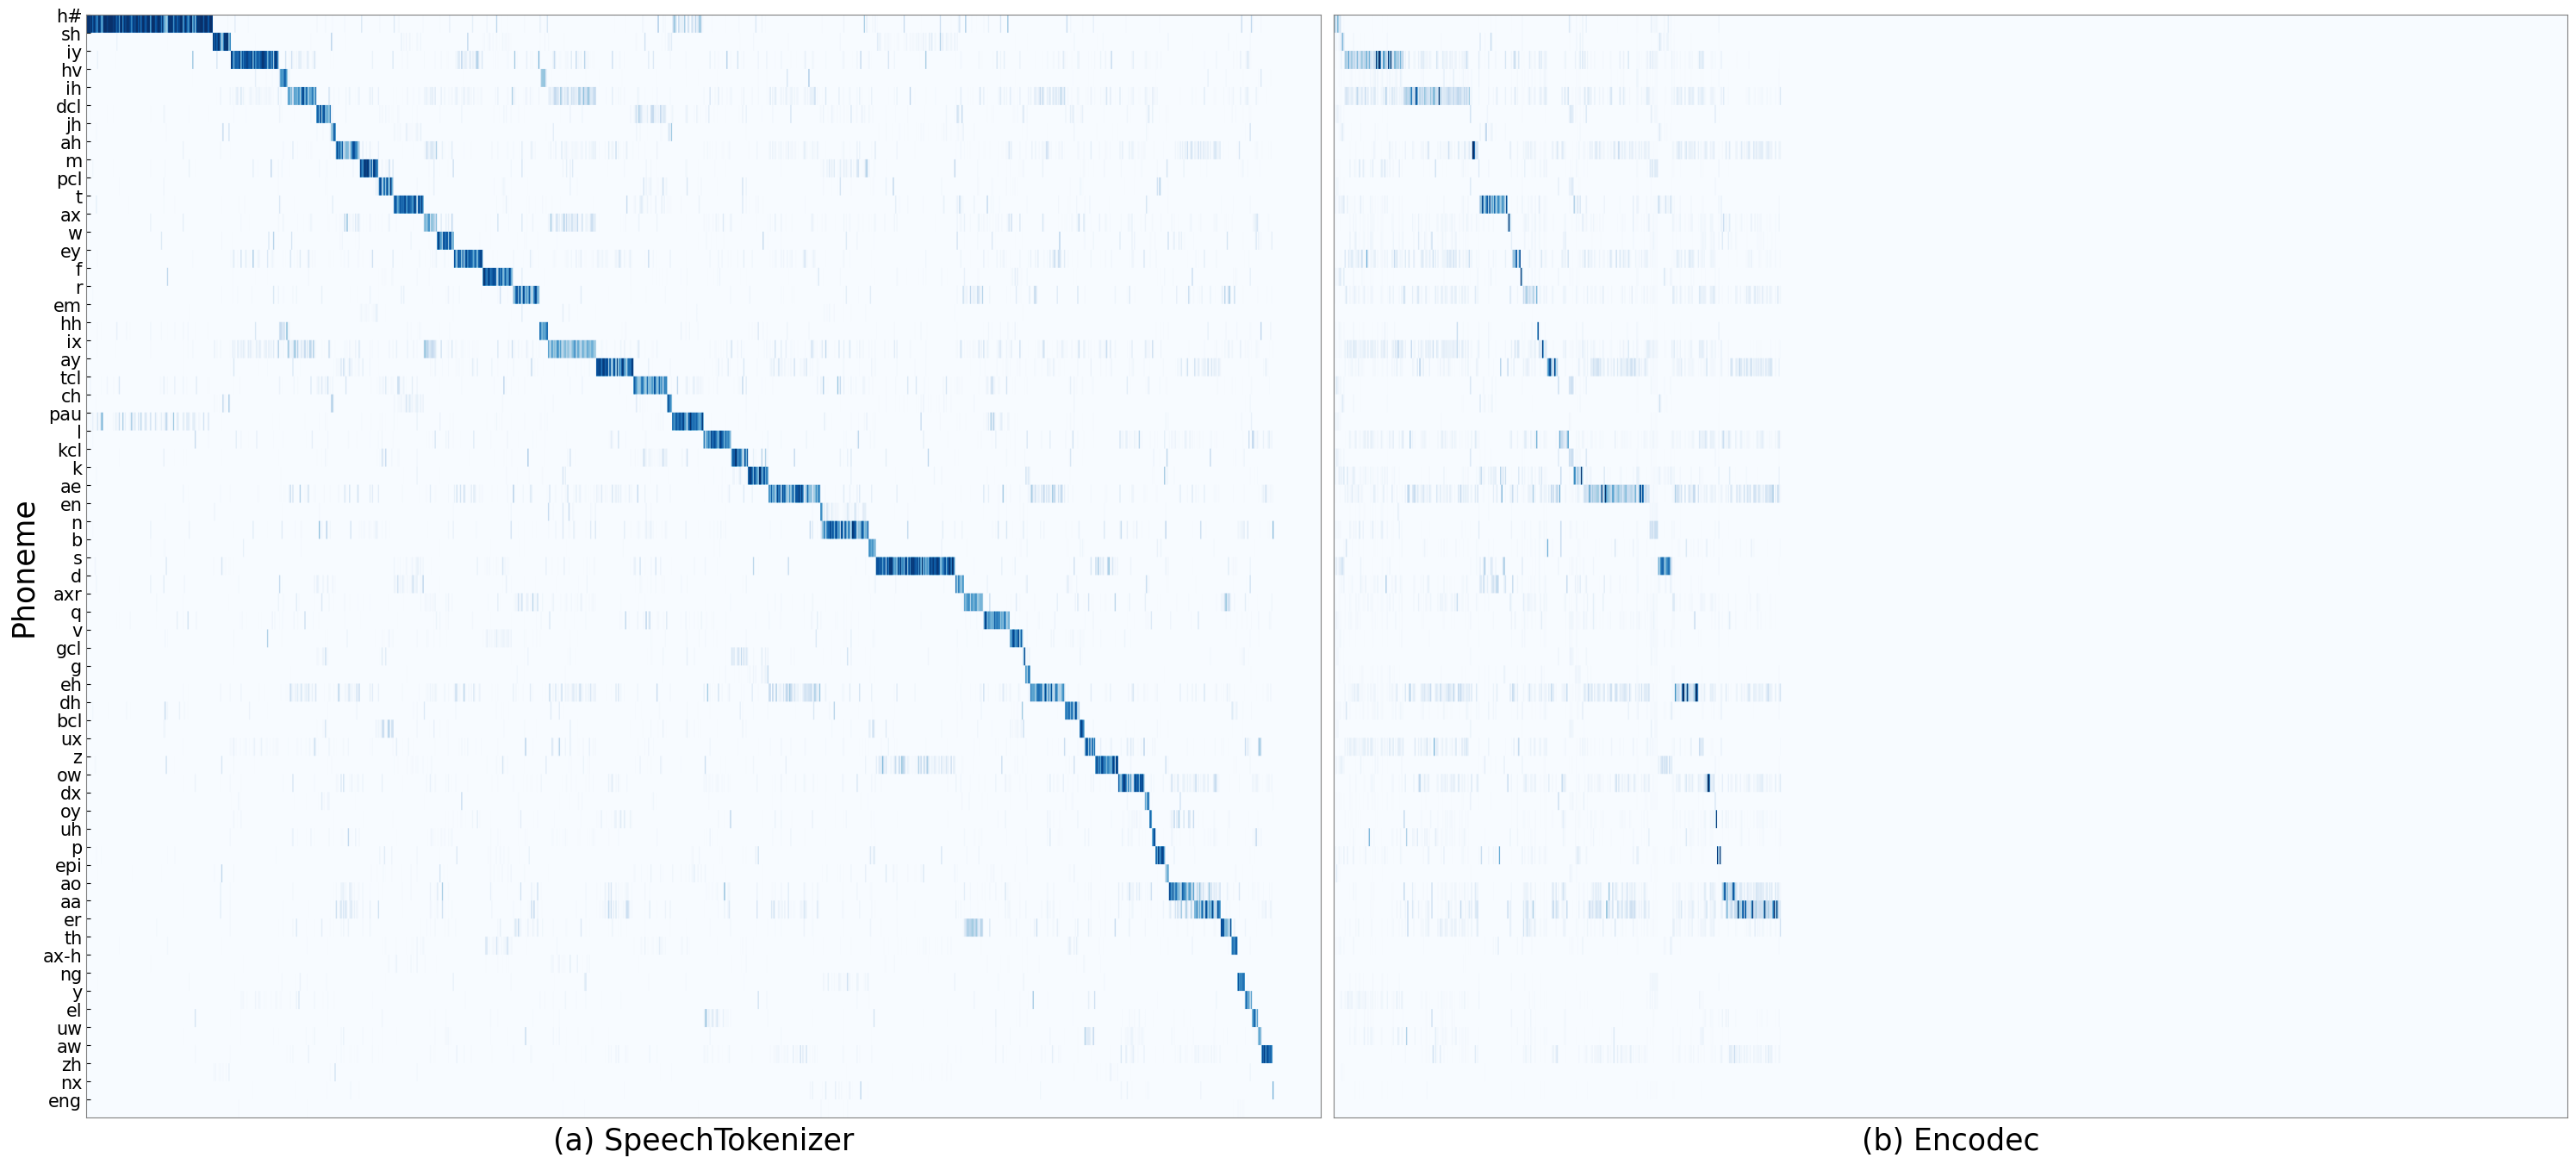
\includegraphics[width=1\textwidth]{Figures/phone_code_coef2.png} 
    \caption{Visualization of the conditional probability $P(\text{phoneme}|\text{code})$ on TIMIT train set. The y-axis is the phoneme set and the x-axis is the codewords of the first RVQ layer sorted by the most correlated phoneme.}%\Phone purity}
    \label{fig:phone_purity} 
\end{figure*}


% \begin{table*}[t]
%     \setlength{\belowcaptionskip}{-0.2cm}
%     % \renewcommand{\arraystretch}{1.2}
%     \Large
%     \centering
%     \resizebox{0.7\textwidth}{!}{
%     \begin{tabular}{lc|ccc}
%         \toprule
%         Tokenizer &   & Phone Purity & Code Purity & PNMI  \\
%         \midrule
%         HuBERT & KM500 & & &  \\
%         EnCodec & RVQ-1 & 0.29 & 0.24 & 0.28 \\
%         \method & RVQ-1 &  0.67 & 0.10 & 0.71 \\
%         \bottomrule
%     \end{tabular}}
%     \caption{PNMI of different discrete speech representation.
%     }
%     \label{tab:pnmi}
% \end{table*}

\begin{table*}[h]
    \setlength{\belowcaptionskip}{-0.2cm}
    % \renewcommand{\arraystretch}{1.2}
    \Large
    \centering
    \resizebox{0.4\textwidth}{!}{
    \begin{tabular}{lc|ccc}
        \toprule
        Tokenizer &  & PNMI$\uparrow$  \\
        \midrule
        HuBERT & KM500 &  0.43 \\
        EnCodec & RVQ-1 & 0.28 \\
        \method & RVQ-1 & 0.71 \\
        \bottomrule
    \end{tabular}}
    \caption{PNMI of different discrete speech representation.
    }
    \label{tab:pnmi}
\end{table*}